\documentclass[tikz,border=6pt]{standalone}
\usepackage{amsmath,amssymb}
\usepackage{xcolor}
\definecolor{accent}{HTML}{A13D2C}
\definecolor{accent2}{HTML}{2B5F6B}
\definecolor{muted}{HTML}{5A564F}
\definecolor{panel}{HTML}{F8F6F0}
\definecolor{linecol}{HTML}{D8D2C4}
\definecolor{astroblue}{HTML}{1B4F72}
\definecolor{ink}{HTML}{1E1C1A}
\usetikzlibrary{calc,arrows.meta}
\usepackage[T1]{fontenc}\usepackage{newpxtext,newpxmath}  % same fonts as the notes
\begin{document}
% Counting encounters. Left: a star system of radius R with a star crossing it on a straight path.
% Right: the same system seen along the path. The path is a point at the centre, each field star's distance
% from it is its impact parameter b, and the stars passed at b to b+db lie in the shaded ring.
% Field stars placed on a golden-angle spiral (deterministic, uniform in projected area).
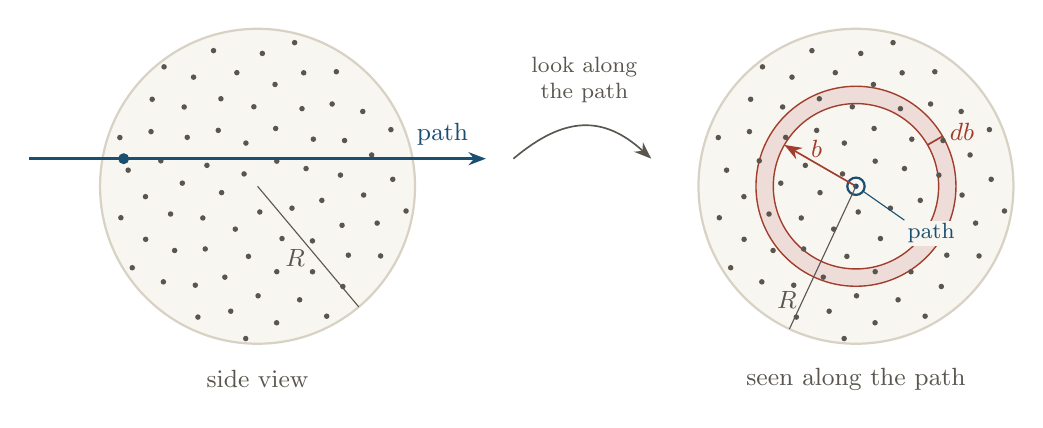
\begin{tikzpicture}[>={Stealth[length=2.2mm]}, font=\small]
  \def\R{2.0}
  % ---- left: side view
  \fill[panel] (0,0) circle (\R);
  \draw[linecol, line width=0.8pt] (0,0) circle (\R);
  \foreach \k in {1,...,70} {
    \pgfmathsetmacro{\rr}{\R*0.97*sqrt(\k/70)}
    \pgfmathsetmacro{\aa}{mod(\k*137.508,360)}
    \fill[muted] (\aa:\rr) circle (0.035);
  }
  \draw[astroblue, line width=1.1pt, ->] (-2.9,0.35) -- (2.9,0.35);
  \node[astroblue, anchor=south west] at (1.9,0.4) {path};
  \fill[astroblue] (-1.7,0.35) circle (0.07);
  \draw[muted] (0,0) -- (-50:\R) node[midway, below left, inner sep=1pt] {$R$};
  \node[muted] at (0,-2.45) {side view};
  % arrow to the end-on view
  \draw[muted, ->, line width=0.6pt] (3.25,0.35) .. controls (3.9,0.9) and (4.4,0.9) .. (5.0,0.35);
  \node[muted, align=center, font=\footnotesize] at (4.15,1.35) {look along\\the path};
  % ---- right: end-on view
  \begin{scope}[xshift=7.6cm]
    \fill[panel] (0,0) circle (\R);
    \draw[linecol, line width=0.8pt] (0,0) circle (\R);
    \def\b{1.05}\def\db{0.22}
    \fill[accent!18, even odd rule] (0,0) circle (\b+\db) (0,0) circle (\b);
    \draw[accent, line width=0.5pt] (0,0) circle (\b) (0,0) circle (\b+\db);
    \foreach \k in {1,...,70} {
      \pgfmathsetmacro{\rr}{\R*0.97*sqrt(\k/70)}
      \pgfmathsetmacro{\aa}{mod(\k*137.508,360)}
      \fill[muted] (\aa:\rr) circle (0.035);
    }
    % the path seen end-on
    \draw[astroblue, line width=0.8pt] (0,0) circle (0.11);
    \fill[astroblue] (0,0) circle (0.035);
    \draw[accent, line width=0.6pt, ->] (0,0) -- (150:\b) node[pos=0.55, above, inner sep=2pt] {$b$};
    \draw[accent, line width=0.6pt] (30:\b) -- (30:\b+\db);
    \node[accent, anchor=west, inner sep=1pt] at ($(30:\b+\db)+(0.05,0.05)$) {$db$};
    \draw[muted] (0,0) -- (-115:\R) node[pos=0.8, left, inner sep=2pt] {$R$};
    \draw[astroblue, line width=0.4pt] (-35:0.12) -- (-35:0.75);
    \node[astroblue, anchor=north west, font=\footnotesize, inner sep=1pt, fill=panel] at (-35:0.75) {path};
    \node[muted] at (0,-2.45) {seen along the path};
  \end{scope}
\end{tikzpicture}
\end{document}
